\chapter{Property Data in the Compressed Graph}%
\label{chp:graph-metadata}

\section{Introduction}

In \cref{chp:graph-dataset} we introduced the \SWHGD{}, a corpus made available
in relational formats suitable for large-scale analysis through scale-out
processing on large Big Data clusters.
In \cref{chp:graph-compression}, we proposed a method to compress the graph to
fit a few hundred gigabytes to efficiently run shared-memory algorithms on a
single machine.
These two approaches are designed to be complementary: scale-out processing is
particularly suited for embarrassingly parallel workflows and can process
terabytes of data in a few minutes with the appropriate scale factor; in-memory
graph compression can run more complex algorithms exploiting the recursive
structure of the graph (traversals, connected components, etc.) in a relatively
cheap way, albeit with longer runtimes of a few hours to a few days.

However, this latter approach is more limited in the kinds of data it can
exploit. The compressed graph only contains the topological structure (nodes
and arcs) of the graph, whereas the graph dataset in relational format can be
used to study the entire \emph{property graph} of development history, i.e.,
not only the graph structure of the dataset but also the properties associated
with each node and edge (e.g., commit messages, timestamps, file names, etc.).
Because of this, recursive graph queries cannot use graph properties during
their traversals. This can be worked around by performing graph queries
without using the properties themselves, then \emph{joining} the results with
data from the relational property graph, but this can be significantly more
expensive and time-consuming.
As an example, let us consider the following query:

\textbf{Query 1}: \emph{Given a blob object, find the earliest revision in
which this blob can be found anywhere in its source code tree.}

If the commit timestamp property can be accessed ``on the fly'' during graph
traversal, this query can be answered in a rather straightforward manner: for
each revision in the transitive closure of the blob in the transposed graph,
find the one with the lowest timestamp. However, if these properties are only
available externally, the process is more involved: it requires returning the
entire transitive closure from the blob, then joining it with the timestamps,
which can require transferring very large amounts of nodes to join with the
timestamps (up to significant fractions of the entire graph, e.g., for the
empty file), before finally filtering on the highest timestamp found.

The added complexity gets even worse when the traversed edges are conditional
on the properties themselves. Consider the following query:

\textbf{Query 2}: \emph{Given a snapshot, find all unique blobs which were
present at the path \allowbreak\texttt{src/test/README.txt} at any point in its
development history.}

With direct access to the properties of the graph, the algorithm is again
straightforward: (1) traverse the revision history (2) for each revision,
follow the given path in its source tree (3) add the destination blob to the
resulting set if not present. This only requires following a single path of
fixed depth for each source code tree, for a time complexity of $O(|R|)$ where
$R$ is the set of revisions in the transitive closure of the snapshot. In
contrast, when the file and directory names of the graph edges are not directly
accessible, one needs to return the \emph{entire transitive closure} of the
snapshot in $O(|N|)$ to later join this data with the graph properties, and use
these to filter the nodes matching the condition in the query.

Whether the compressed graph is used only for selecting artifacts for the
purpose of performing subsequent scale-out analyses on the extracted data, or
directly used for the analyses themselves, having direct access to the graph
properties from the compressed format would significantly improve the
efficiency of more complex graph queries.
In this chapter, we look at ways to bridge this potency gap between the two
formats by enabling access to node and edge properties from the compressed
graph.

\section{SWHID mappings}

The most basic property of the graph is the \acrfull{SWHID} of each node, their
unique identifier in the archive. They are of prime importance to be able to
relate the nodes being manipulated in the compressed representation with the
archived artifacts themselves.

The input of the graph compression pipeline is a list of nodes and edges
referenced by their \glspl{SWHID} in a format described in
\cref{sec:edges-format}.  As detailed in \cref{sec:compression-pipeline}, this
pipeline works by mapping each unique \gls{SWHID} to a set of consecutive
integers $\{0,\ldots,N-1\}$, where $N$ is the number of nodes in the graph by
computing a \emph{minimal perfect hash function}~\cite{GOVFSCF}.  After this
hashing step, the \gls{SWHID} information is lost, and all the nodes are
subsequently referred to as their integer identifier from the contiguous set.
To restore the ability to associate the graph nodes with the objects they refer
to, we need to construct mapping functions that allow us to translate between
integer node IDs and \glspl{SWHID} in both directions.

\subsection{SWHID $\to$ Node ID}%
\label{sec:swhid2node}

The natural way to map \glspl{SWHID} to the compressed node IDs is to reuse the
minimal perfect hash function which was used to map the nodes in the first
place.
This hash function is stored as a \texttt{graph.mph} file (which weighs
around 5\,GiB for the 2020-12-15 version of the graph) and can translate the
input \glspl{SWHID} to node IDs in this set. However, during the compression
pipeline the graph is \emph{reordered} to achieve better compression results,
as described in \cref{sec:compression-pipeline}. When compressing with the
\gls{LLP} algorithm, the graph is even reordered twice: once for the initial
BFS-based compression, and then once for the LLP-based compression. As a
consequence of these reorderings, the node IDs obtained from feeding
\glspl{SWHID} to the \gls{MPH} function no longer correspond to their matching
output nodes.

A byproduct of the compression pipeline are ``order files'' which define
the \emph{permutations} of each reordering step. Their on-disk format is a
binary array of integers in which the integer at position $x$ is $p(x)$ where
$p$ is the permutation of the reordering step. As such, the \gls{SWHID} $\to$
node ID mapping can be obtained by composing the \gls{MPH} with the subsequent
reorderings. As a preliminary step, if the graph was permuted multiple times
(as is the case for \gls{LLP}), we compose the \texttt{.order} files to keep a
single permutation $p_G$, which corresponds to the resulting permutation of
successively applying all the compression permutations of the graph:

\begin{itemize}
    \item For BFS-based compression: $p_G(i) = p_{\mathrm{BFS}}(i)$
    \item For LLP-based compression:
        $p_G(i) = (p_{\mathrm{LLP}} \circ p_{\mathrm{BFS}})(i)$
\end{itemize}

This lowers memory usage by reducing the number of order files necessary for
the translation to node IDs. For reference, an order file representing a
permutation for 19.3 billion nodes (the size of the 2020-12-15 dataset) weighs
around 145\,GiB ($\approx 19.3 \times 10^9 \times 8 \times \frac{1}{2^{30}}$
for 64-bit node IDs).
This composed permutation (or ``graph permutation'', as it represents how the
graph is permuted from the original order of the nodes given by the hashing
function) is stored as a \texttt{graph.order} file in the same format as the
input permutations.

Then, the mapping function for the \gls{SWHID} $\to$ node ID direction can be
defined from the \gls{MPH} and the composed permutation:

\[\mathit{swhid2node}(s) = p_G(\mathit{mph}(s))\]

In other words, getting the node ID associated with a given input \gls{SWHID}
$s$ can be done through the following two-step process:

\begin{enumerate}
    \item Hash the \gls{SWHID} $s$ using the \gls{MPH} function loaded from the
        \texttt{graph.mph} file to obtain $k_0$, the node ID from the initial
        graph order.
    \item Take the image of $k_0$ from the graph permutation stored in the
        \texttt{graph.order} file to obtain the node ID $k$.
\end{enumerate}

The storage space taken by the entire mapping is the on-disk size of the
permutation plus the on-disk size of the hash function, which is $\approx
150$\,GiB in the 2020-12-15 dataset. This is comparable to the size of the
graph itself (134\,GiB for the forward graph only). This size could be reduced
by compressing the \texttt{.order} file, which could be achieved by reducing
the number of bits used for each entry in the permutation to the bare minimum
necessary to represent an integer in the set of node IDs. Doing so would come
at the cost of some inefficiency due to the overhead of correcting word
misalignment, which would potentially be negligible.  For the same example, the
estimated size would then be:

\[
    n \times \left\lceil{\frac{\log_2(n)}{8}}\right\rceil\,\mathrm{bytes}
    = 19.3 \times 10^9 \times
        \left\lceil{\frac{\log_2(19.3 \times 10^9)}{8}}\right\rceil
        \times \frac{1}{2^{30}}
    \approx 90\,\mathrm{GiB.}
\]

\subsection{Node ID $\to$ SWHID}%
\label{sec:node2swhid}

Now that we are able to easily convert \glspl{SWHID} to their corresponding
node IDs in the compressed graph, we can build a \emph{reverse mapping} which
allows us to retrieve the \gls{SWHID} preimage of any node ID found in the
compressed graph. This reverse mapping is the inverse function
$\mathit{node2swhid}$ (= $\mathit{swhid2node}^{-1}$) of the mapping
described in the previous section.

This function is relatively easy to represent on disk for two reasons. First,
its input domain is a contiguous set of integers $\{0,\ldots,N-1\}$, which
means the function does not require any hashing scheme to associate images to
its inputs; they can simply be stored as a contiguous array. Second, because
the images are \glspl{SWHID} they all have a fixed size, which facilitates
random access in the array.

This reverse mapping is stored in a file called \texttt{graph.node2swhid.bin},
a binary file containing a contiguous binary sequence of records, each record
representing a \gls{SWHID}. The binary format used to represent a \gls{SWHID}
as a 22-byte long byte sequence is constituted of:

\begin{itemize}
    \item 1 byte for the namespace version, represented as a C \emph{unsigned
        char}
    \item 1 byte for the object type as the integer value of a software
        artifact type enum (0 = content, 1 = directory, 2 = origin, 3 =
        release, 4 = revision, 5 = snapshot), represented as a C \emph{unsigned
        char}
    \item 20 bytes for the SHA-1 digest represented as a byte sequence.
\end{itemize}

This mapping can be generated relatively straightforwardly by (1) allocating a
binary file of $22 \times n$ bytes, (2) iterating on the list of all the
\glspl{SWHID} used to compress the graph, (3) for each \gls{SWHID}, getting
$k$, its image node ID, using the mapping described in \cref{sec:swhid2node},
(4) writing the 22 bytes binary record representing the \glspl{SWHID} at the
offset $22 \times k$ in the binary file.

Once this mapping is written to disk, the \gls{SWHID} of a node $k$ can be
retrieved by simply reading the 22-bytes binary record at index $22 \times k$.
A \texttt{graph.node2swhid.bin} file mapping 19.3 billion node IDs (the size of
the 2020-12-15 dataset) to their corresponding \glspl{SWHID} weighs
around 395\,GiB ($\approx 19.3 \times 10^9 \times 22 \times \frac{1}{2^{30}}$).

\subsection{Domain checking}

One caveat of the approach described in \cref{sec:swhid2node} to map
\gls{SWHID} $\to$ node ID is that it does not do any kind of checking on its
input domain; an unknown/invalid \gls{SWHID} will be accepted by the hash
function, which will return an arbitrary integer in its image
$\{0,\ldots,N-1\}$ instead of throwing an error. This is problematic for some
use cases: if the compressed graph is exposed as an API, it needs to be able to
reject queries using unknown \glspl{SWHID}, instead of silently computing a
garbage result on the wrong input node without any way for the user to notice.

While it is possible to externally check whether a \gls{SWHID} is present in
the Software Heritage archive by querying its API, this is not sufficient for
this use case. The compressed graph is not built incrementally but is instead a
\emph{static} export of the state of the archive at a given point in time. This
means that all nodes added to the archive during the time period between
the graph compression and the present are unknown to the compressed graph.

One option to add checks to the input domain would be to add \textbf{signing} to
the \gls{MPH} function. By associating a signature of $w$ bits to each input
key of the \gls{MPH} function, it is able to detect input strings which were
not in the original key set. This approach is probabilistic, and false
positives are possible with a probability of {\Large $\frac{1}{2^w}$}. While
this is useful to catch bugs, a probabilistic approach does not allow us to
systematically fall back when encountering an unknown \gls{SWHID} unless using
very large signatures. These can also dramatically increase the size of the
hashing function: for the 2020-12-15 dataset, a 32-bit signatures increases its
size from 5\,GiB to 72\,GiB while still allowing a false positive every 4
billion \gls{SWHID} on average, which is less than a quarter of the number of
objects in the graph.

Instead, we consider another option based on \textbf{round-trips} on the
mapping from \cref{sec:swhid2node} and reverse mapping from
\cref{sec:node2swhid}.  Because both mappings are bijections which are
the inverse of one another, it follows that for every \gls{SWHID} $s$ in the
input key set of the \gls{MPH}, $\mathit{node2swhid}(\mathit{swhid2node}(s)) =
s$.  In contrast, if $s$ \emph{is not} in the input domain,
$\mathit{swhid2node}(s)$ will return an arbitrary node, and
$\mathit{node2swhid}(\mathit{swhid2node}(s))$ will then return a random
\gls{SWHID} \emph{from the input domain}, which thus cannot be equal to $s$.

Given this, it is possible to create a function which maps \gls{SWHID} $\to$
node IDs \emph{with domain checking} by performing this ``round-trip'' to
verify that the node is in the input domain, and returning an error otherwise:

\[
    \mathit{swhid2nodeCheck}(s) =
    \begin{cases}
        \mathit{swhid2node}(s) &
        \text{\textbf{if}}~\mathit{node2swhid}(\mathit{swhid2node}(s)) = s,\\
        \text{-1}            & \text{\textbf{otherwise.}}
    \end{cases}
\]

\section{Node properties}%
\label{sec:node-properties}

After having restored the association between the nodes in the graph and their
archive identifiers, we now move to storing node properties \emph{other} than
\glspl{SWHID}.
For the reasons outlined in \cref{sec:node2swhid}, mapping nodes to properties
in external storage is generally a relatively simple feat. Because the node IDs
in the compressed graph are consecutive integers in the range
$\{0,\ldots,N-1\}$, mapping each node to a given property is equivalent to
creating a random-access list of properties, in which the property found at
index $k$ is the one associated with the node $k$.

The best way to achieve this depends on the type and characteristics of each
property, detailed in \cref{sec:relational-model}. We can use these to organize
the properties in different categories, for each of which we describe an
implementation for compact on-disk storage in this section.

\subsection{Node types}%
\label{sec:mapping-types}

In \cref{sec:compression-comp-scope} we already mentioned keeping \emph{node
types} in memory, i.e., whether a node is a blob, directory, revision, etc.
Node types have a special status because they are necessary for almost all
kinds of analyses on the graph as they allow determining at runtime which
kinds of objects are being traversed. They are also
already present as part of the textual identifiers of the nodes themselves,
being one of the fields in \gls{SWHID}. For that reason, we systematically
load this node type mapping in memory along with the graph, contrary to the
other mappings which have to be loaded on demand.
This mapping is implemented very efficiently as a bit array indexed by integer
node identifiers, with records of only 3 bits per node (as there are 6 node
types in total), which amounts to around 7\,GiB of RAM for the 2020-12-15
graph.

\subsection{Integer properties}%
\label{sec:mapping-integers}

The following properties are simple integers, either 16, 32 or 64 bits:

\begin{itemize}
    \setlength\itemsep{0em}
    \item \texttt{content.length}: size of a blob in bytes
    \item \texttt{revision.date}: timestamp of when a revision was authored
    \item \texttt{revision.date\_offset}: timezone offset of when a revision
        was authored
    \item \texttt{revision.committer\_date}: timestamp of when a revision was
        committed
    \item \texttt{revision.committer\_date\_offset}: timezone offset of when a
        revision was committed
    \item \texttt{release.date}: timestamp of when a release was authored
\end{itemize}

All the dates can be represented as a 64-bit timestamp storing the number of
nanoseconds since the Unix epoch. The timezone information is stored as a
16-bit integer representing the timezone offset with UTC.

Storing these integer properties in property files is done in a similar way
to storing permutations in order files, which we described in
\cref{sec:swhid2node}. Because integers have a fixed width, these properties
can be stored in a relatively straightforward manner as binary array of
integers in which the $k$th integer corresponds to the value of the property
for node $k$.  The resulting property files have a size of {\Large $n \times
\frac{w}{8}$}, where $n$ is the number of nodes in the graph, and $w$ the
number of bits of the integer field (16, 32 or 64). For the 2020-12-15 export,
these bit sizes correspond respectively to property files of size 35\,GiB,
71\,GiB and 145\,GiB.

This could further be improved if the nodes of each type were stored
contiguously, as it would allow us to store integers in a contiguous array
without having holes for nodes of irrelevant types. Using such a typed graph
would have various advantages in terms of property storage and locality-based
compression, and is left as a future work.

\subsection{Persons}%
\label{sec:mapping-persons}

The following properties represent ``persons'', which are stored as records
containing a full name and an email address.\footnote{Like software projects,
persons are ontologically complex objects and cannot be solely described by a
name and an email: people have multiple emails, change names, can misspell
their own name, etc. Past works have attempted to map authorship information to
a canonical concept of ``persons'' by merging duplicate information to single
identities~\cite{wiese2016mailing, zhu2019empirical}. For the purposes of this
thesis, we call ``person'' a unique pair of full name and email address, and
leave identity deduplication in the hands of the users of the platform.}

\begin{itemize}
    \setlength\itemsep{0em}
    \item \texttt{revision.author}: author of a revision
    \item \texttt{revision.committer}: committer of a revision
    \item \texttt{release.author}: author of a release
\end{itemize}

Those fields are natively represented as byte sequences in the relational
format.  However, two factors come into play to figure out the best way to
store these properties for the compressed graph. First, there are considerably
fewer unique persons than there are objects referring to persons: only 42
million persons in the 2021-03-23 graph export, whereas there are 2 billion
objects containing person fields (revisions and releases), which highlights the
usefulness of having some deduplication of unique authors. Second, as discussed
in \cref{sec:relational-model}, the research use cases we want to support are
not those exploiting the names and e-mails of the authors themselves (which we
anonymize anyway), but rather those trying to relate identical authors, e.g.,
for the purpose of analyzing the structure of social coding networks.

In consequence, the only data we actually want to provide for this property is
a unique identifier of a given person, which will then be used in place of the
full name and email and can be compared across different objects.
Because the graph is static, persons can be mapped to integers in the range
$\{0,\ldots,N-1\}$ where $N$ is the total number of persons referenced in the
graph artifacts. This is once again achieved with the use of an \gls{MPH}: we
first extract the list of unique persons in the graph, then compute a minimal
perfect hash on the full names and e-mails to associate each person to a unique
integer. The integer array is then stored in binary format using the method
described above for regular integer fields. There is no need to build and
provide a reverse mapping for the anonymization reasons explained above.

\subsection{Text}%
\label{sec:mapping-text}

Finally, the most complex type of node fields in the property graph is the
textual type, or rather, arbitrary sequences of bytes. The following properties
use this byte sequence type:

\begin{itemize}
    \setlength\itemsep{0em}
    \item \texttt{revision.message}: descriptive message of a revision
    \item \texttt{release.message}: descriptive message of a release
\end{itemize}

Because these fields need to be properly readable (i.e., one should actually be
able to get the entire byte sequence from a node, contrary to persons), there
is not much optimization to be done for this case. We can use an arbitrary
on-disk string list which maps each node ID to its property value, as long as
it allows random access. For this purpose we use the
\texttt{FrontCodedStringBigList}
class\footnote{https://dsiutils.di.unimi.it/docs/it/unimi/dsi/big/util/FrontCodedStringBigList.html}
from the \texttt{dsiutils} library\footnote{https://dsiutils.di.unimi.it/} used
in the WebGraph framework. It contains an index table to efficiently jump to
the $k$th bytestring in the array.
For the 2021-03-23 export, the total size of all the byte strings we need to
store is 159\,GiB, which is a manageable amount.  However,
\texttt{FrontCodedStringBigList} objects have to be loaded entirely in memory,
which can be a significant memory burden. Improving this by making it possible
to memory-map this data structure from disk is left open as a future
implementation direction.

\section{Edge properties}%
\label{sec:mapping-edge-labels}

While most properties in the graph are associated with the objects themselves,
some properties are associated with the relationships between them, which we
call ``edge properties''. While they are relatively few, we expect them to be
of crucial importance for most analysis workflows, as they include file and
directory names which are a key property used in software mining; file
extensions in particular are one of the most relevant properties that
researchers use to find artifacts of interest. The complete list of edge
properties in the relational schema which we want to make available from the
compressed graph is as follows (a more detailed description of these properties
are available in \cref{sec:relational-model}):

\begin{itemize}
    \setlength\itemsep{0em}
\item \texttt{snapshot\_branch.name} (binary): name of a snapshot branch
    (on snapshot $\to\ast$ edges)
\item \texttt{directory\_entry.name} (binary): name of a directory entry
    (on directory $\to\ast$ edges)
\item \texttt{directory\_entry.perms} (int): permissions of a directory
    entry (on directory $\to\ast$ edges)
\end{itemize}

\subsection{Data structure}%
\label{sec:label-data-structure}

As we have seen, attaching properties to graph nodes using an external
on-disk mapping is relatively straightforward: because the nodes are mapped to
a contiguous integer range, in all cases the data structure only needs to map
this range to a set of properties, which can be done efficiently in most cases.
However, for properties attached to the graph \emph{edges}, doing so gets
technically harder: the input domain of the mapping is the sparse adjacency
matrix of the entire graph, which cannot be compactly represented in a naive
data structure.

To solve this issue, the WebGraph framework provides an experimental set of
libraries\footnote{\url{https://webgraph.di.unimi.it/docs/it/unimi/dsi/webgraph/labelling/package-summary.html}}
under \texttt{webgraph.labelling} which implements arc labeling, i.e.,
associating arbitrary properties to the graph edges. The basic principle for
the serialization of labels (the objects storing the edge properties) using
this system is twofold.

First, all labels are written to a \texttt{graph.labels} file in the order
obtained by iterating on all edges of the graph.  As a reminder, WebGraph
stores the outgoing arcs of each node as an ordered adjacency list, and all the
nodes in the graph are ordered from $0$ to $N-1$.  Enumerating all nodes
and all outgoing arcs of each enumerated node in the compressed graph
yields a natural ordering for all edges stored in the graph, which can be
then be followed to store the labels on disk.

Second, a \texttt{graph.labeloffsets} file is used to index the offsets of the
arc labels. This file can be seen as an integer array which associates a node
$k$ with the position in the \texttt{graph.labels} file from which the labels
of its outgoing arcs can be read. This offset file allows random access to the
labels on the outgoing arcs of a given source node.

In other words, given a node $k$, it is possible to lookup in constant time
a position $p_k$ from the offset file, then iterate on all outgoing edges
of $k$ while reading the arc labels file starting from $p_k$ to
successively retrieve all labels of the outgoing arcs of $k$. It is however not
possible to get the specific arc label of a $k_1 \to k_2$ edge in constant
time, as WebGraph does not allow access to arbitrary edges in constant time;
instead, all outgoing edges of $k_1$ need to be iterated along with their
labels until $k_2$ is encountered in the adjacency list, which has an average
complexity of $O(d_{\mathrm{out}})$, where $d_{\mathrm{out}}$ is the average
out-degree of the nodes in the graph.

% TODO: maybe an illustration would be welcome here.

The labels themselves can be in any arbitrary self-contained format, as they
are read sequentially from the label file and deserialized using a custom
function. The simplest format for an arc label is to associate a record of a
fixed number of bits to each arc. This poses an important challenge for
our use case. Consider a directory with two files having different names but
an identical content, for example two empty files, as shown in
\cref{fig:multiple-labels}. In our data model, this would be represented as two
nodes (the directory and the blob corresponding to the empty file) and two
edges from the first to the second node (one for each file entry). In the
compressed graph however, due to the copy-list model of compression, these
nodes would only be linked together by a single arc, to which we cannot
associate a single file name.

\begin{figure}
    \centering
    \begin{tikzpicture}[font=\footnotesize]
        \node [style=directory] (0) at (0, 0) {};
        \node [style=content] (1) at (4, 0) {ø};
        \draw [style=arrow, bend left] (0) to node [above, sloped]
            {\texttt{.gitkeep}} (1);
        \draw [style=arrow, bend right] (0) to node [above, sloped]
            {\texttt{ISSUES.txt}} (1);

    \end{tikzpicture}
    \caption{Two directory entries with different names pointing to the same
    blob (the empty file). This is stored as a single edge in the compressed
    graph, and thus has to be represented with multiple labels per arc.}%
    \label{fig:multiple-labels}
\end{figure}

% \footnotetext{The astute reader might notice that a software project with an
% empty bug list is rather unlikely; it is indeed used here as a highly
% hypothetical example.}

To represent this possibility of having multiple file names for a single arc,
in the case of multiple relationships between two identical nodes, we cannot
rely on having one fixed-size label for each arc. Instead, each arc label is
stored as a \emph{list} of records, each record representing one relationship
between two nodes, which allows us to circumvent the single arc constraint.
A version of this design which can store lists of fixed-size integers as the
arc labels is implemented as the \texttt{FixedWidthIntListLabel} class in the
WebGraph framework; we extended this class to allow for lists of larger (up to
64 bits) fixed width labels in a new class, \texttt{FixedWidthLongListLabel}.

\subsection{Label format}
\label{sec:label-format}

Each record in the label list described above represents one relationship
between two nodes. Because there are $O(|E|)$ labels to store, it is important
to find a compact representation for these labels so as to avoid requiring
inordinate amounts of storage space.

For the sake of simplicity, and to avoid keeping multiple label files around,
we can find a uniform representation for both snapshot branches and directory
entries. Directory entries are constituted of a binary name and an integer for
permissions, whereas snapshot branch labels only contain a binary name; we can
thus represent all labels as a pair of a binary sequence field and an integer
field, which happens to always be an unused value for snapshot branches.

Moreover, we do not actually need to store permissions as arbitrary integers:
file permissions are normalized when extracted from the archive and can only
take one of five values (plus a special ``none'' value for the special case of
snapshot branches).  Normalized permissions can therefore be stored in a 3 bits
enumeration:

\begin{table}[H]
    \centering
\begin{tabular}{c c c l}
    \textbf{Value} & \textbf{Bits} & \textbf{Unix permission} & \textbf{Entry type} \\
    0 & 000 & --- & None (used for snapshot branches) \\
    1 & 001 & \texttt{0o100644} & Regular file \\
    2 & 010 & \texttt{0o100755} & Executable file (\texttt{+x}) \\
    3 & 011 & \texttt{0o120000} & Symbolic link \\
    4 & 100 & \texttt{0o040000} & Directory \\
    5 & 101 & \texttt{0o160000} & Revision (e.g., git submodules)
\end{tabular}
\end{table}

Regarding file names and branch names, the naive implementation would be to
write the full byte sequence representing the entry name in each label. As an
order of magnitude, the total size of all binary entry names in the
2021-03-23 graph export is 4.0\,TiB, which is impractical to store on disk.
However, this can be drastically improved by compressing identical file names
together, as (1) the nature of our \gls{VCS} data model duplicates a lot of
relationships between objects which only changed their contents, but not their
names, and (2) entry names are massively reused in general (e.g.,
\texttt{README.md}, \texttt{refs/heads/master}, \texttt{main.c}).
While there are 225 billion different directory \emph{entries} in the
latest export, there are only 2.3 billion different \emph{entry names}.
By only storing each unique entry name once, we can cut down the 4\,TiB
estimation of the naive approach down to only 62\,GiB, which is far more
manageable (especially for fast access as it can be stored in a single SSD).

For that purpose, we can once again use a \gls{MPH} function to associate each
label with a unique integer in the range $\{0, \ldots, N_L-1\}$ where $N_L$ is
the total number of unique names used in arc labels. Then, we can use a reverse
mapping to retrieve a given byte sequence from its associated integer using a
\texttt{FrontCodedStringList} as detailed in \cref{sec:node-properties}.  Here,
a new trade-off appears: front-coded string lists are particularly efficient at
compressing similar strings when they are \emph{ordered}, i.e., when successive
strings in the list share a common prefix, as the front-coding can be used to
compress the prefix across different values. However, standard \gls{MPH}
functions map their input to integers in an arbitrary order, which nullifies
the advantages of the front-coding. Some \gls{MPH} functions, called
\emph{monotone minimal perfect hashing functions}, can be used to map their
input in an order-preserving fashion~\cite{belazzougui2008theory}, although the
resulting functions are generally larger and have a slower hashing throughput.
An implementation of such a function is implemented as the
\texttt{LcpMonotoneMinimalPerfectHashFunction} in the Sux4J
framework\footnote{\url{https://sux.di.unimi.it/}}.

We empirically benchmarked the storage performance and hashing speed of three
different techniques for label name mapping on the 2020-12-15 graph:

\begin{enumerate}
    \item \label{itm:label-gov3-fcl}
        \textbf{Standard \gls{MPH} with unsorted front-coded string list}: this
        approach uses a standard \gls{MPH} which does not preserve the order of
        its input keys, negating the compression benefits of front-coded string
        lists.
    \item \label{itm:label-gov3-pfcl}
        \textbf{Standard \gls{MPH} with permuted sorted front-coded string
        list}: this approach uses a standard \gls{MPH} which does not preserve
        the order. However, the front-coded string list is stored by
        lexicographical order, which allows it to benefit from front-coding
        compression. To map the results of the hash function to the order in
        the list, a \emph{permutation array} is used, as described in
        \cref{sec:swhid2node}.
    \item \label{itm:label-lcp-fcl}
        \textbf{Monotone \gls{MPH} with sorted front-coded string list}: this
        approach uses a monotone \gls{MPH} which maps its input in an
        order-preserving fashion (but has a larger size and lower hashing
        rate), and a sorted front-coded string list.
\end{enumerate}

\begin{table}[b]
    \centering
    \caption{Benchmark results of three different techniques to hash and build
        a reverse mapping of the set of snapshot branch names and directory
        entry names.}%
    \label{tab:label-mph-benchmark}
    \begin{tabular}{c l r r r}
        \textbf{Option} & \textbf{Implementation} & \textbf{MPH size} & \textbf{Total size} & \textbf{Hashing rate} \\ \hline
        \ref{itm:label-gov3-fcl} & Standard MPH + unsorted FCL & 0.6\,GiB & 172\,GiB & 521 k lines/s \\
        \ref{itm:label-gov3-pfcl} & Standard MPH + permuted FCL & 0.6\,GiB & 124\,GiB & 521 k lines/s \\
        \ref{itm:label-lcp-fcl} & Monotone MPH + sorted FCL & 5.7\,GiB & 114\,GiB & 511 k lines/s
    \end{tabular}
\end{table}

The results of this benchmark are shown in \cref{tab:label-mph-benchmark}. As
can be seen in the results, the front-coded compression on sorted lists
drastically reduces the size of the reverse mapping: 172\,GiB for the unsorted
list, 108\,GiB for the sorted list, for a total compression ratio of 1.59.
Among the two options with a sorted front-coded string list,
option~\ref{itm:label-gov3-pfcl} adds to that amount a 16\,GiB permutation
array for a total of 124\,GiB, while option~\ref{itm:label-gov3-pfcl} increases
the size of the hash function from 0.6\,GiB to 5.7\,GiB for a total of
114\,GiB. Because the hashing rate is practically identical between the two
different hashing functions, and using a monotone \gls{MPH} makes the label
writing pipeline simpler, we pragmatically oriented ourselves towards that
latter option.

Armed with efficient encoding mechanisms for the two fields of arc labels
(permission enumeration and monotonically hashed entry name identifiers), we
can specify the format for each record: a $3 +
\left\lceil{\log_2(N_L)}\right\rceil$ bits long integer ($= 35$ bits for
the 2021-03-23 graph) encoding the permission value in its three lower bits and
the index of the entry name in the front-coded string list in its upper bits.

\subsection{Label compression pipeline.}

\begin{figure}
    \centering
    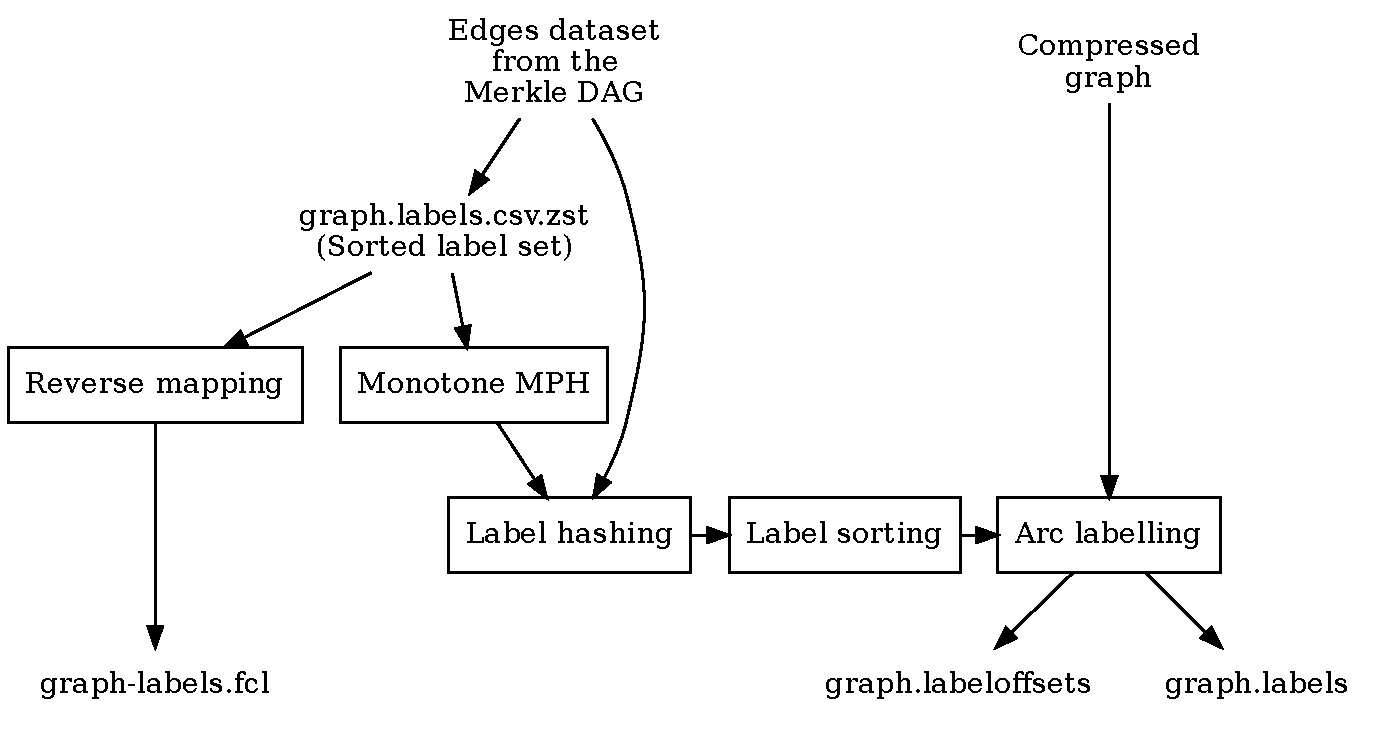
\includegraphics[width=\textwidth]{img/graph-properties/label-compression}
    \caption{Label compression pipeline}%
    \label{fig:label-compression-pipeline}
\end{figure}


Having settled the format for arc labels, we can now describe a compression
pipeline to generate the on-disk labels from the input dataset. As a reminder,
in \cref{sec:edges-format} we described the input edges format for graph
compression, a CSV file of edges in the format:

\texttt{<source node> <destination node> [<entry name> [<permissions>]]<CR>}

\paragraph{Label set extraction}
The first step of the pipeline is to extract the set of unique label names
(directory entry and snapshot branch names) from the edges dataset. We iterate
on the entire set of edges and extract the third field (entry name) when it is
present, then use this feed as an input to the GNU \texttt{sort(1)} command
with the \texttt{-u} option, to only keep unique entries. We then compress the
output using the Zstandard algorithm~\cite{collet2015zstd}, and obtain a
compressed and sorted set of all the unique label names in the graph.

\paragraph{Monotone MPH}
Using the set of label names, we can generate the hashing function to convert
entry names to and from the set of integers $\{0, \ldots, N_L-1\}$ using a
Monotone \gls{MPH} as described in \cref{sec:label-format}. The
\texttt{LcpMonotoneMinimalPerfectHashFunction} class takes the sorted set of
labels $L$ as an input, and generates an $h_L$ function which converts any
given entry name from the set $L$ to its rank in the sorted list of label
names.

\paragraph{Reverse mapping}
In order to access the value of any given label name from its integer rank in
$O(1)$ time, we then build an efficient on-disk map using the
\texttt{FrontCodedStringBigList} class by giving it the sorted list of labels
as an input, which stores them efficiently using front-coding compression while
allowing fast random access. This map $m_L$ is the inverse function
of $h_L$ over its input domain: $\forall l \in L,~m_L(h_L(l)) = l$.

\paragraph{Label hashing}
As explained in \cref{sec:label-data-structure}, the labels have to be stored
in the natural order of edges in the compressed graph. This compressed order is
different from the order observed in the edges dataset, which is
arbitrary and depends on the export process. We thus need to hash the node
\gls{SWHID} using the \texttt{swhid2node} function on both the source and the
destination, and the $h_L$ function on the label byte strings in order to
reorder them in the final compressed order.

To illustrate this process, given the following edges dataset (in the format
described in \cref{sec:edges-format}):

\begin{minted}{text}
<src> <dst> <label_name> <perms>
swh:1:snp:4548a5… swh:1:rev:0d6834… cmVmcy9oZWFkcy9tYXN0ZXI=
swh:1:dir:05faa1… swh:1:cnt:a35136… dGVzdC5j 420
swh:1:dir:05faa1… swh:1:dir:d0ff82… dGVzdA== 16384
\end{minted}

We (1) hash and permute the source and destination nodes using
$p_G(\mathit{mph}(s)$, and (2) monotonically hash the labels using $h_L(l)$, to
obtain the identifiers which will be used in the compressed graph:

\begin{minted}{text}
pG(mph(<src>) pG(mph(<dst>)) hL(<label_name>) <perms>
4421 14773 154
1877 21441 134 420
1877 14143 141 16384
\end{minted}

\paragraph{Label sorting}
Then, we can reorder the list of edges to match the order of edges in the
compressed graph.
We use GNU \texttt{sort(1)} with a large in-memory buffer and temporary
space on disk to obtain the sorted edges. Sort is called with the \texttt{-n
-k1,1 -k2,2} options to numerically sort on each field:

\begin{minted}{text}
1877 14143 141 16384
1877 21441 134 420
4421 14773 154
\end{minted}

This sorting step is extremely intensive in time and memory: because there are
more than 220 billion edges to sort in the latest dataset and because the
sorting algorithm has a complexity of $O(|E| \times \log(|E|))$, the process
can take entire weeks, terabytes of disk space and hundreds of gigabytes of
RAM.

Since the lines that need to be sorted are fixed-width numbers, other
sorting methods can be used to reduce memory usage. The
\texttt{bsort}\footnote{\url{https://github.com/pelotoncycle/bsort}} program
implements an in-place radix sort, which avoids storing terabytes of temporary
buffers on-disk. To use it, we store the result of the hashing step in binary
format, one record per line. To avoid spending time sorting on the leading
zeros, the source and destination node IDs are written in a fixed size byte
array of size $w = \left\lceil{\frac{\log_2(N_L)}{8}}\right\rceil$ bytes. The
total record is of size $2 \times w + 8 + 4$, to store respectively the source
and destination nodes, the 64-bit label identifier and the 32-bit permission
integer. The \texttt{bsort} program is then called with the options \texttt{-k
<w*2> -r <w*2+8+4>} to specify respectively the record size and the number of
leading bytes used for sorting.

We benchmarked the label sorting pipeline using \texttt{sort} and
\texttt{bsort} on a smaller graph of around 350 million edges, and obtained
similar results ($12'30''$ for \texttt{sort}, $11'30''$ for \texttt{bsort}).
We have not yet been able to conclusively determine whether one sorting method
would be significantly faster than the other on larger input files. Both
sorting methods are thus made available, configurable by the user as a command
line option.

\paragraph{Arc labeling}
Finally, with the ordered list of edges in numerical format, we can write the
labels to the \texttt{graph.labels} file and its offset to the
\texttt{graph.labeloffsets} file. For this, we need to traverse the graph edges
in order, and synchronize the traversed edges with the stream of labelled
edges, skipping unlabeled edges in the graph. This process is shown in
\cref{algo:label-writing} and has a complexity of $O(|E|)$.

\begin{algorithm}[htb]
    \begin{algorithmic}
        \Function{WriteLabels}{$G,~S_E$}
        \State $l \gets \{-1, -1, -1, -1\}$ \Comment{Placeholder edge line}
        \ForAll{$n \in G$} \Comment{For all the nodes in the graph}
            \State $w \gets 0$ \Comment{Number of bits taken by the labels of
            the outgoing edges}
            \ForAll{$e \in \Call{out}{n}$} \Comment{For all outgoing edges from
            $n$}
                \State $A \gets$ empty array \Comment{Array of labels for
                this outgoing edge}
                \While {($l_\mathit{src}, l_\mathit{dst}) < (e_\mathit{src},
                    e_\mathit{dst})$} \Comment{Synchronize traversal and label
                    stream}

                    \If {($l_\mathit{src}, l_\mathit{dst}) = (e_\mathit{src},
                        e_\mathit{dst})$} \Comment{Traversed edge is in sync with label
                        stream}
                        \State add $(l_\mathit{entry}, l_\mathit{perms})$ to $A$
                    \EndIf

                    \If {$S_E$ at \texttt{EOF}} \Comment{Exit case for end of stream}
                        \State \textbf{break}
                    \Else
                        \State $l \gets \Call{NextLine}{S_E}$
                    \EndIf
                \EndWhile
                \State $b \gets \Call{SerializeLabelArray}{A}$
                \State $w \gets w + \Call{Length}{B}$
                \State Append $b$ to \texttt{graph.labels}
            \EndFor
            \State Append $w$ to \texttt{graph.labeloffsets}
        \EndFor
        \EndFunction
    \end{algorithmic}

    \caption{Write the labels from the sorted edge streams to a compressed
    representation. This algorithm works by synchronizing two traversals: the
sorted edges of the graph $G$ and the sorted edges from the numerical stream of
labelled edges $S_E$.}%
    \label{algo:label-writing}
\end{algorithm}

\section{Memory considerations}

We export graph properties as a set of files which live next to the compressed
graph, one file per property. The specific formats used for these property
files have been detailed in the previous sections. In this section we discuss
time and memory considerations surrounding access to these properties from the
compressed graph.

\subsection{Direct loading and memory-mapping}

As one might expect, in the graph of software development the vast majority of
storage space is occupied by the properties themselves; the structure of nodes
and arcs is just a small portion of the total size. This highlights an
important speed/memory trade-off: it is highly unlikely that the entire
property graph can be realistically stored in memory in the same way as the
graph structure itself. Therefore, it makes sense for the properties to be
stored offline by default (presumably on disk) and then loaded on demand
when the analysis requires it.

There are different ``levels'' of loading external data on-demand, each with
its own memory requirements:

\begin{enumerate}
    \item Loading the entire mapping from disk to main memory. This immediately
        increases the main memory usage by the size of the mapping, which
        guarantees that property access is bounded by the speed of the physical
        RAM with no disk I/O involved.
    \item Mapping the file in virtual memory with \texttt{mmap(1)}. This
        delegates the possibility to cache large sections of the file in main
        memory to the kernel when enough physical RAM is available; however,
        when a segment of the file is accessed without having been cached,
        accessing the mapping will trigger a page fault and require disk I/O,
        slowing down access times.
        Here, performance becomes dependent on (a) the amount of available RAM
        and (b) how well the kernel is able to predict access patterns (to the
        extent that they are actually predictable and not random seeks).
        The main advantage of this method is to avoid reserving large amounts
        of physical RAM for the mapping.
    \item Seeking to a given position in an offline on-disk file. This makes
        property access fully I/O bound, with each read requiring a system
        call. The I/O operation need not translate to a physical disk read, as
        the kernel can still cache some sections of the file in main memory.
        This method has minimal advantages compared to memory-mapping for large
        files, so we generally do not provide it as an option for property
        access.
\end{enumerate}

From the level of the graph compression framework, it makes sense to put the
direct loading and memory-mapping methods at the disposal of the end-user, so
that they can tune on-demand property loading to their specific workloads and
hardware. We thus try to provide, for the mappings that support it, two loading
methods: \texttt{load} and \texttt{loadMapped} to implement options (1) and
(2), respectively.
Each mapping can be loaded at any point during runtime. It is generally more
efficient to directly load smaller mappings which are often used in RAM (e.g.,
the node type mapping should generally always be loaded directly), whereas
larger files like integer arrays should be memory-mapped if the amount of
physical RAM is a binding constraint on the hardware.

\subsection{Sharing mapped data across processes}%
\label{sec:cachemount}

Often, multiple processes can be working on the same data (mappings or the
graph itself), for instance when running different experiments on the same
graph. This is problematic in terms of RAM usage when using direct memory
loading, as the same data of potentially hundreds of gigabytes is loaded in
memory twice. Memory-mapping can be used to avoid storing redundant data in
RAM, but comes at a cost of potentially slower I/O as the data is no longer
guaranteed to be loaded in main memory and is reliant on kernel heuristics.

We propose another approach to share data across two different compressed graph
processes while loading it \emph{directly in RAM}, through the use of the
\texttt{swh graph cachemount} command. By copying graph data to a
\emph{tmpfs}~\cite{snyder1990tmpfs} not backed by a disk swap, we can force the
kernel to load it entirely in RAM. Subsequent memory-mappings of the files
stored in the tmpfs will simply map the data stored in RAM to virtual memory
pages, and return a pointer to the in-memory structure.

From a user perspective, using the \texttt{cachemount} command can be done in
just a few steps: (1) choose the graph data and mappings which need to always
be loaded in main memory to be shared by the compressed graph processes; (2)
call the \texttt{cachemount} command with the list of relevant files, which
copies them in the tmpfs located at \texttt{/dev/shm}; (3) memory-map the files
from the graph processes using the \texttt{loadMapped} method, which returns a
virtual mapping to the in-RAM structure.

\section{Walkthrough}

We conclude this chapter by briefly demonstrating how to use graph properties
from the Java API of the \texttt{swh.graph} framework using the mapping
techniques described in the sections above.

The graph itself can be loaded either with memory-mapping or direct loading; it
is however recommended to always load it using memory-mapping while using the
\texttt{cachemount} command described in \cref{sec:cachemount} to share data
between several \texttt{swh.graph} processes. A third option is to load the
graph in ``offline mode'', without loading the edges themselves in memory; this
disables random node access and only allows the graph to be iterated
sequentially.

\begin{minted}{java}
SwhGraph g1 = SwhGraph.load(graphPath);  // direct loading
SwhGraph g2 = SwhGraph.loadMapped(graphPath);  // memory mapping
SwhGraph g3 = SwhGraph.loadOffline(graphPath);  // offline mode
\end{minted}

The \texttt{SwhGraph} object automatically loads the node type maps described
in \cref{sec:mapping-types} with direct loading, as this mapping is
comparatively small. The type of each node can then be looked-up using
\texttt{getType}:

\begin{minted}{java}
// Printing all node types
NodeIterator it = graph.nodeIterator();
while (it.hasNext()) {
    long k = it.nextLong();
    // returns the node type (among {ORI, SNP, REL, REV, DIR, CNT})
    SwhNode.Type t = graph.getType(k);
    System.out.println(t);
}
\end{minted}

The node ID $\leftrightarrow$ \gls{SWHID} mappings described in
\cref{sec:swhid2node} and \cref{sec:swhid2node} are provided through
\texttt{NodeIdMap}, a wrapper of the \gls{MPH} function, the \texttt{.order}
files for the permutation, and the binary file containing the reverse mapping.
By default, the \gls{MPH} function is loaded with direct loading, while the
other bigger files are memory-mapped.

\begin{minted}{java}
// Loading SWHID <-> node ID maps
NodeIdMap m = new NodeIdMap(graphPath, graph.numNodes());

// Printing all node SWHIDs
NodeIterator it = graph.nodeIterator();
while (it.hasNext()) {
    long k = it.nextLong();
    // returns the SWHID of the given node
    SwhNode.Type swhid = m.getSWHID(k);
    System.out.println(swhid);
}
\end{minted}

Other node properties like integer timestamp arrays can be either loaded
directly or using memory-mapping.

\begin{minted}{java}
// Direct loading
long[][] revTimestamps = (long[][]) BinIO.loadLongsBig(
    graphPath + "-rev_timestamps.bin");

// Memory-mapping (alternatively)
LongBigList revTimestamps = ByteBufferLongBigList.map(
    new FileInputStream(graphPath + "-rev_timestamps.bin").getChannel());

// Printing all commit timestamps
NodeIterator it = graph.nodeIterator();
while (it.hasNext()) {
    long k = it.nextLong();
    if (graph.getType(k) == Node.Type.REV) {
        long timestamp = BigArrays.get(revTimestamps, k)
        System.out.println(graph.getSWHID(k) + ": " + timestamp);
    }
}
\end{minted}

Finally, properties on the graph edges described in
\cref{sec:mapping-edge-labels} require the use of a graph wrapper class,
\texttt{ArcLabelledImmutableGraph}, which provides an API to seamlessly read
arc labels from the \texttt{graph.labels} file while iterating on the graph
edges. From there, the on-disk front-coded string array can be loaded and used
to retrieve textual label names from their hashed identifier:

\begin{minted}{java}
// Load graph, node mapping and label name reverse mapping
ArcLabelledImmutableGraph graph = BitStreamArcLabelledImmutableGraph.loadMapped(
    graphPath + "-labelled");
NodeIdMap nodeMap = new NodeIdMap(graphPath, graph.numNodes());
FrontCodedStringBigList labelNameMap = (FrontCodedStringBigList) BinIO.loadObject(
    graphPath + "-labels.fcl");

// Print all edges and their labels
ArcLabelledNodeIterator it = graph.nodeIterator();
while (it.hasNext()) {
    long srcNode = it.nextLong();
    ArcLabelledNodeIterator.LabelledArcIterator s = it.successors();
    long dstNode;
    while ((dstNode = s.nextLong()) >= 0) {
        SwhLabel[] labels = (SwhLabel[]) s.label().get();
        if (labels.length > 0) {
            for (SwhLabel label : labels) {
                System.out.format(
                    "%s %s %s %d\n",
                    nodeMap.getSWHID(srcNode),
                    nodeMap.getSWHID(dstNode),
                    labelNameMap.get(label.filenameId),
                    label.permission);
            }
        }
    }
}
\end{minted}
